\chapter{First-order response functions}
\label{chp:first-order_response}

In the approximation scheme introduced by \textcite{Zmuidzinas2012ARCMP} and discussed in Section~\ref{sec:theory.perturbation}, the quasiparticle occupancy $\qpoccupancy(\energy)$ is treated as given.
For calculating the response of a KID, the interesting properties of the superconducting state depend on both the gap and the occupancy; however, the gap also depends on the occupancy and must be determined in a self-consistent manner.
To treat this complication approximately, consider only quantities that are proportional to $\qpoccupancy$, which is used as a small parameter, and write equations that are self-consistent to first order.

For a thermal (Fermi-Dirac) occupancy
$\qpoccupancy(\energy, \temperature) = [\exp(\energy / \kb \temperature) + 1]^{-1}$
at a temperature such that
$\kb \temperature / \gap_\zerotemp \ll 1$,
we can make the approximation
$\qpoccupancy(\energy, \temperature) \approx \exp(-\energy / \kb \temperature)$ as long as there are no states too far below the gap.
This allows the integrals of the first-order quantities to be performed analytically.

\subsubsection{Gap energy}

To derive the first-order response function for the gap, start with the BCS self-consistency equation~\autocite{Tinkham2004}
\begin{equation}
1 
  =
  \bcspotential \sum_{\vwvec} \frac{1 - 2 \qpoccupancy_{\vwvec}}{\left( \blochenergyf_{\vwvec}^2 + \gap^2 \right)^{1/2}},
\end{equation}
where
$\blochenergyf_{\vwvec} = \blochenergy_{\vwvec} - \blochenergy_\fermi$
is the Bloch state energy measured from the Fermi energy $\blochenergy_\fermi$,
and $\qpoccupancy_{\vwvec}$ is the occupancy of the quasiparticle state with energy
$\energy_{\vwvec} = \left( \blochenergyf_{\vwvec}^2 + \gap^2 \right)^{1/2}$.
The sum is over all wavevectors $\vwvec$ such that
\begin{equation}
\left| \blochenergyf_{\vwvec} \right|
  <
  \blochenergyf_\cutoff
  \sim
  \blochenergyf_\debye,
\end{equation}
the Debye energy.
Because $\blochenergy_\debye \gg \gap \gg \kb \temperature$, we have
$\qpoccupancy(\energy = \blochenergyf_\debye) = 0$
and we can take the limits of the corresponding integral to be infinite:
\begin{equation}
1
  =
  \ssdos \ucvolume \bcspotential
  \int_{-\infty}^\infty \dd{\blochenergyf}
  \frac{1 - 2 \qpoccupancy \left(\energy = [\blochenergyf^2 + \gap^2]^{1/2} \right)}{(\blochenergyf^2 + \gap^2)^{1/2}}.
\end{equation}

Expand around the zero-temperature value $\gap_\zerotemp$, using
$\delta\gap = \gap - \gap_\zerotemp$:
\begin{equation}
\frac{1}{(\blochenergyf^2 + \gap^2)^{1/2}}
  =
  \frac{1}{(\blochenergyf^2 + \gap_\zerotemp^2)^{1/2}}
  - \frac{\gap_\zerotemp }{(\blochenergyf^2 + \gap_\zerotemp^2)^{3/2}} \delta\gap
  + \mathcal{O}\left( \delta\gap^2 \right).
\end{equation}
Assume that the occupancy is small so that the term linear in $\qpoccupancy$ is already first-order.
The first-order self-consistency equation is then
\begin{align}
1
  &=
  \ssdos \ucvolume \bcspotential
  \int_{-\infty}^\infty \dd{\blochenergyf}
  \left( \frac{1}{(\blochenergyf^2 + \gap_\zerotemp^2)^{1/2}}
  - \frac{\gap_\zerotemp}{(\blochenergyf^2 + \gap_\zerotemp^2)^{3/2}} \delta\gap
  - \frac{2 \qpoccupancy \left(\energy = [\blochenergyf^2 + \gap_\zerotemp^2]^{1/2} \right)}{(\blochenergyf^2 + \gap_\zerotemp^2)^{1/2}}
  \right) \\
\therefore \qquad
0
  &=
  \delta\gap \int_{-\infty}^\infty \dd{\blochenergyf} \left(
  \frac{\gap_\zerotemp}{(\blochenergyf^2 + \gap_\zerotemp^2)^{3/2}}
 + \frac{2 \qpoccupancy \left(\energy = [\blochenergyf^2 + \gap_\zerotemp^2]^{1/2} \right)}{(\blochenergyf^2 + \gap_\zerotemp^2)^{1/2}}
 \right),
\end{align}
since the left-hand side and the first term define $\gap_\zerotemp$.
With $z = \blochenergyf / \gap_\zerotemp$,
\begin{equation}
\frac{1}{\gap_\zerotemp} \int_{-\infty}^\infty \frac{\dd{z}}{(z^2 + 1)^{3/2}}
  =
  \frac{2}{\gap_\zerotemp},
\end{equation}
so the shift in the gap is
\begin{equation}
\delta\gap
  =
  -\frac{\gap_\zerotemp}{2} \int_{-\infty}^\infty \dd{\blochenergyf}
   \frac{2 \qpoccupancy \left(\energy = [\blochenergyf^2 + \gap_\zerotemp^2]^{1/2} \right)}{(\blochenergyf^2 + \gap_\zerotemp^2)^{1/2}}.
\end{equation}
Use the fact that the integrand is even and change variables to
$\energy = (\blochenergyf^2 + \gap_\zerotemp^2)$:
\begin{equation}
\delta\gap
  =
  - 2 \gap_\zerotemp \int_{\gap_\zerotemp}^\infty \dd{\energy}
   \frac{\qpoccupancy (\energy)}{(\energy^2 - \gap_\zerotemp^2)^{1/2}}.
\end{equation}
Thus, the first-order response function is
\begin{equation}
\responseqpoccupancy_\gap(\energy)
  =
  -\frac{2 \gap_\zerotemp}{(\energy^2 - \gap_\zerotemp^2)^{1/2}}
  =
  -\frac{2 \gap_\zerotemp \qprdos_\zerotemp(\energy)}{\energy},
\label{eqn:first-order_response.responseqpoccupancy_gap}
\end{equation}
where
$\qprdos_\zerotemp = \energy (\energy^2 - \gap_\zerotemp^2)^{-1/2}$
is the reduced density of states at zero temperature.

For a thermal occupancy, using the above low-temperature approximation and the dimensionless variable
$z = \energy / \gap_\zerotemp$,
the first-order shift in the gap is
\begin{align}
\braket{\responseqpoccupancy_\gap}{\qpoccupancy(\temperature)}
  &=
  -2 \gap_\zerotemp \int_{\gap_\zerotemp}^\infty \dd{\energy}
  \frac{\exp(-\energy / \kb \temperature)}{(\energy^2 - \gap_\zerotemp^2)^{1/2}} \\
  &=
  -2 \gap_\zerotemp \int_1^\infty \dd{z} \frac{\exp(-\gap_\zerotemp z / \kb \temperature)}{(z^2 - 1)^{1/2}} \\
  &=
  -2 \gap_\zerotemp K_0 \left( \frac{\gap_\zerotemp}{\kb \temperature} \right),
\label{eqn:first-order_response.responseqpoccupancy_gap_thermal}
\end{align}
where $K_0$ is the zero-order modified Bessel function of the second kind.
\todo[inline]{Replace link when figure is included.}
%Figure~\ref{fig:gap_versus_temperature} shows this expression and the full BCS expression that is also valid at higher temperatures.

\subsubsection{Quasiparticle density}

The first-order response function for the quasiparticle density (or number) follows simply from the definitions.
With the same notation and expanded limits as above,
\begin{equation}
\qpdensity
  =
  2 \ssdos \int_{-\infty}^{\infty} \dd{\blochenergyf}
  \qpoccupancy \left( \energy = (\blochenergyf^2 + \gap^2)^{1/2} \right).
\end{equation}
As above, the integrand is already first-order so we neglect the shift in the gap and set $\gap = \gap_\zerotemp$.
Changing variables and using the symmetry,
\begin{equation}
\qpdensity
  \approx
  \braket{\responseqpoccupancy_{\qpdensity}}{\qpoccupancy}
  =
  \int_{\gap_\zerotemp}^{\infty} \dd{\energy}
  \frac{4 \ssdos \energy}{(\energy^2 - \gap_\zerotemp^2)^{1/2}}
  \qpoccupancy(\energy).
\end{equation}
Including the cutoff in the density of states, the first-order response function is simply
\begin{equation}
\responseqpoccupancy_{\qpdensity}(\energy)
  =
  4 \ssdos \qprdos_\zerotemp(\energy),
\label{eqn:first-order_response.responseqpoccupancy_qpdensity}
\end{equation}
which we would have obtained by naively replacing $\gap$ with $\gap_\zerotemp$ in Equation~\ref{eqn:qpdensity}.

For a thermal occupancy, with the usual approximation, we have
\begin{equation}
\braket{\responseqpoccupancy_{\qpdensity}}{\qpoccupancy(\temperature)}
  =
  4 \ssdos \int_{\gap_\zerotemp}^{\infty} \dd{\energy}
  \frac{\energy \exp(-\energy / \kb \temperature)}{(\energy^2 - \gap_\zerotemp^2)^{1/2}}.
\end{equation}
\todo[inline]{Flesh out using Abramowitz and Stegun}
This integral is done by \textcite{Thomas2015SUST}, who give
\begin{equation}
\qpdensity(\temperature)
  =
  4 \ssdos \gap_\zerotemp
  K_1(\gap_\zerotemp / \kb \temperature)
  \approx
  4 \ssdos \gap_\zerotemp
  \left( \frac{\pi \kb \temperature}{2 \gap_\zerotemp} \right)^{1/2}
  \exp \left( -\frac{\gap_\zerotemp}{\kb \temperature} \right),
\label{eqn:first-order_response.qpdensity_thermal}
\end{equation}
which is Equation~\ref{eqn:qpdensity_thermal} in the main text.

\subsubsection{Complex conductivity}

\begin{figure}[htb]
\centering
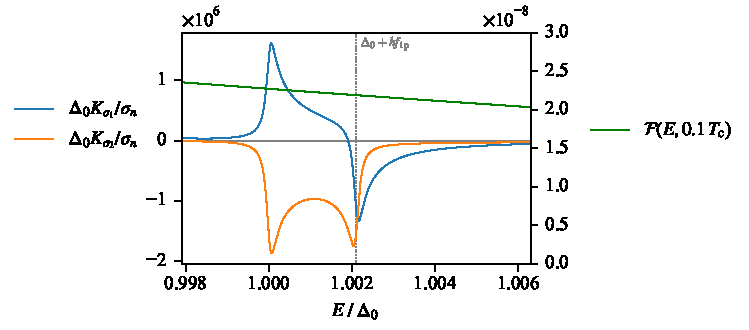
\includegraphics[width=\textwidth]{first-order_response/responseqpoccupancy_conductivity_f_1p.pdf}
\caption
[The first-order response functions for the real and imaginary parts of the conductivity at $\freadout_\singlepol$.]
{The first-order response functions for the real and imaginary parts of the conductivity at $\freadout_\singlepol = \SI{0.1}{GHz}$ versus energy in units of the gap, and a thermal occupancy.
The left axis shows Equations~\ref{eqn:responseqpoccupancy_reconductivity} and~\ref{eqn:responseqpoccupancy_imconductivity} multiplied by constants to make them dimensionless.
For display, the density of states factors have been broadened using $\mitrovic / \gap_\zerotemp = 0.0002$.
The right axis shows a thermal occupancy at a typical KID operating temperature.
Figure~\ref{fig:responseqpoccupancy_conductivity_f_mc} shows the same quantities at a much higher frequency, where the peaks in the response functions are farther apart.}
\label{fig:responseqpoccupancy_conductivity_f_1p}
\end{figure}

In calculating the first-order response functions for the complex conductivity at the readout frequency $\freadout$ we can assume that $\planck \freadout / 2 \gap \ll 1$.
The expressions for $\responseqpoccupancy_{\reconductivity}$ and $\responseqpoccupancy_{\imconductivity}$ are plotted for two different frequencies in Figures~\ref{fig:responseqpoccupancy_conductivity_f_mc} and~\ref{fig:responseqpoccupancy_conductivity_f_1p}.

For the real part of the conductivity, start with Equation~\ref{eqn:mattisbardeen1}.
In this limit, only the first term is present:
\begin{equation}
\frac{\reconductivity(\freadout)}{\normalconductivity}
  =
  \frac{2}{\planck \freadout} \int_\gap^\infty \dd{\energy}
  \left[ \qpoccupancy(\energy) - \qpoccupancy(\energy + \planck \freadout) \right]
  \frac{\energy^2 + \gap^2 + \planck \freadout \energy}
  {[\energy^2 - \gap^2]^{1/2} [(\energy + \planck \freadout)^2 - \gap^2]^{1/2}}.
\label{eqn:mattisbardeen1subgap}
\end{equation}
For brevity, and to anticipate possible broadening, rewrite the integrand using the density of states:
\begin{equation}
\frac{\reconductivity(\freadout)}{\normalconductivity}
  =
  \frac{2}{\planck \freadout} \int_\gap^\infty \dd{\energy}
  \left[ \qpoccupancy(\energy) - \qpoccupancy(\energy + \planck \freadout) \right]
  \qprdos(\energy) \qprdos(\energy + \planck \freadout)
  \left(1 + \frac{\gap^2}{\energy (\energy + \planck \freadout)} \right).
\end{equation}
The entire integrand is proportional to the occupancy, so
$\reconductivity(\temperature = 0) = 0$
and we may neglect the first-order shift in the gap, which would appear at second order, and set
$\gap = \gap_\zerotemp$.
If we write the density of states in the form
$\qprdos_\zerotemp(\energy) = \Re{\energy (\energy^2 - \gap_\zerotemp^2)^{-1/2}}$,
we can change variables in the second term and combine the integrals, setting both lower limits to 0:
\begin{align}
\begin{split}
\frac{\reconductivity(\freadout)}{\normalconductivity}
  &=
  \frac{2}{\planck \freadout} \int_0^\infty \dd{\energy}
  \qpoccupancy(\energy)
  \bigg[
  \qprdos_\zerotemp(\energy) \qprdos_\zerotemp(\energy + \planck \freadout)
  \left(1 + \frac{\gap_\zerotemp^2}{\energy (\energy + \planck \freadout)} \right) \\
  &\hspace{1.3in} - \qprdos_\zerotemp(\energy - \planck \freadout) \qprdos_\zerotemp(\energy)
  \left(1 + \frac{\gap_\zerotemp^2}{(\energy - \planck \freadout) \energy} \right)
  \bigg].
\end{split}
\end{align}
(This change of variables should not cause problems unless there are states far below the gap, close to $\energy = 0$.)
We can now read off the first-order response function:
\begin{equation}
\responseqpoccupancy_{\reconductivity}(\energy)
  =
  \frac{2 \normalconductivity \qprdos_\zerotemp(\energy)}{\planck \freadout}
  \left[
  \qprdos_\zerotemp(\energy + \planck \freadout)
  \left(1 + \frac{\gap_\zerotemp^2}{\energy (\energy + \planck \freadout)} \right)
  - \qprdos_\zerotemp(\energy - \planck \freadout)
  \left(1 + \frac{\gap_\zerotemp^2}{(\energy - \planck \freadout) \energy} \right)
  \right],
\label{eqn:first-order_response.responseqpoccupancy_reconductivity}
\end{equation}
which matches Equation~\ref{eqn:responseqpoccupancy_reconductivity}.
To calculate $\braket{\responseqpoccupancy_{\reconductivity}}{\qpoccupancy(\temperature)}$ for a thermal occupancy  $\qpoccupancy(\temperature)$ at low temperature, start from Equation~\ref{eqn:mattisbardeen1subgap}, and, following \textcite{Barends2009}, change to a dimensionless variable
\begin{equation}
z
  =
  \frac{2}{\planck \freadout} \left( \energy - \gap_\zerotemp + \frac{\planck \freadout}{2} \right).
\end{equation}
Then, using
$D = 2 \gap_\zerotemp / \planck \freadout \gg 1$
so that
$\energy = (\planck \freadout / 2) (z + D - 1)$,
\begin{align}
\begin{split}
\frac{\braket{\responseqpoccupancy_{\reconductivity}}{\qpoccupancy(\temperature)}}{\normalconductivity}
  &=
  2 \sinh \left( \frac{\planck \freadout}{2 \kb \temperature} \right)
  \exp \left( -\frac{\gap_\zerotemp}{\kb \temperature} \right)
  \int_1^\infty
  \exp \left( -\frac{\planck \freadout z}{2 \kb \temperature} \right) \\
  &\hspace{1in} \times  \frac{z^2 + 2 D z + 2 D^2 - 1}{[2 D (z - 1) + (z - 1)^2]^{1/2} [2 D (z + 1) + (z + 1)^2]^{1/2}} \dd{z} \\
  &\approx
  2 \sinh \left( \frac{\planck \freadout}{2 \kb \temperature} \right)
  \exp \left( -\frac{\gap_\zerotemp}{\kb \temperature} \right)
  \int_1^\infty
  \exp \left( -\frac{\planck \freadout z}{2 \kb \temperature} \right)
  \frac{D}
  {(z - 1)^{1/2} (z + 1)^{1/2}} \dd{z}.
\end{split}
\end{align}
The exponential falls off rapidly, so the weight is highest near $z \gtrsim 1$.
We thus neglect all terms in the numerator except $2 D^2$.
In the denominator, $(z - 1)^2$ is negligible near $z = 1$ where the weight is highest.
For $z \approx 2 D$, where $(z \pm 1)^2$ becomes significant, the argument of the exponential is negative and large
$(2 \gap_\zerotemp / \kb \temperature \gg 1)$, so we can also neglect these terms.
In this form, the integral can be done analytically, as above, with the result
\begin{equation}
\frac{\braket{\responseqpoccupancy_{\reconductivity}}{\qpoccupancy(\temperature)}}{\normalconductivity}
  =
  \frac{4 \gap_\zerotemp}{\planck \freadout}
  \exp \left( -\frac{\gap_\zerotemp}{\kb \temperature} \right)
  \sinh \left( \frac{\planck \freadout}{2 \kb \temperature} \right)
  K_0 \left( \frac{\planck \freadout}{2 \kb \temperature} \right).
\label{eqn:first-order_response.responseqpoccupancy_reconductivity_thermal}
\end{equation}

The derivation of the first-order response function for the imaginary part of the conductivity proceeds similarly, starting from Equation~\ref{eqn:mattisbardeen2} with the lower bound appropriate for
$\planck \freadout / 2 \gap < 1$:
\begin{equation}
\frac{\imconductivity}{\normalconductivity}
  =
  \frac{1}{\planck \freadout} \int_{\gap - \planck \freadout}^{\gap} \dd{\energy}
  \left[ 1 - 2 \qpoccupancy(\energy + \planck \freadout) \right]
  \frac{\energy (\energy + \planck \freadout) + \gap^2}
  {[\gap^2 - \energy^2]^{1/2} [(\energy + \planck \freadout)^2 - \gap^2]^{1/2}}.
\label{eqn:mattisbardeen2subgap}
\end{equation}
The occupancy does not appear in the first term, so the zero-temperature value is nonzero.
Using the same dimensionless variables as above,
\begin{align}
\begin{split}
\frac{\imconductivity(\temperature = 0)}{\normalconductivity}
  &=
  \int_{-1}^{1} \frac{\dd{z}}{2}
  \frac{z^2 + 2 D z + 2 D^2 - 1}{[2 D (1 - z) - (1 - z)^2]^{1/2} [2 D (1 + z) + (1 + z)^2]^{1/2}} \\
  &\approx
  \int_{-1}^{1} \dd{z}
  \frac{D / 2}{(1 - z)^{1/2} (1 + z)^{1/2}}.
\end{split}
\end{align}
As before, we retain only the largest term in the numerator.
The integrand is singular at both limits, and we neglect
$(z \pm 1)^2$
in the denominator because the other terms dominate near the limits.
\todo[inline]{Flesh out using A\&S.}
With the substitution $\theta = \arccos(-z)$, we obtain
\begin{equation}
\frac{\imconductivity(\temperature = 0)}{\normalconductivity}
  =
  \frac{\pi \gap_\zerotemp}{\planck \freadout}.
\end{equation}
The second term in Equation~\ref{eqn:mattisbardeen2subgap} is linear in $\qpoccupancy$, so again we set $\gap = \gap_\zerotemp$ in this term.
However, the first term also produces a first-order contribution because the shift in the gap appears at this order:
$\gap = \gap_\zerotemp + \braket{\responseqpoccupancy_{\gap}}{\qpoccupancy}$.
Using Equation~\ref{eqn:first-order_response.responseqpoccupancy_gap}, factoring the second term, and changing limits gives
\begin{align}
\begin{split}
\frac{\imconductivity - \imconductivity(\temperature = 0)}{\normalconductivity}
  &=
\frac{\pi \braket{\responseqpoccupancy_{\gap}}{\qpoccupancy}}{\planck \freadout}
  - \frac{2}{\planck \freadout} \int_{\gap}^{\gap + \planck \freadout} \dd{\energy}
  \qpoccupancy(\energy)
  \frac{(\energy - \planck \freadout) \energy + \gap^2}
  {[\gap^2 - (\energy - \planck \freadout)^2]^{1/2} [\energy^2 - \gap^2]^{1/2}} \\
  &=
  \int_{0}^{\infty}
  \dd{\energy} \qpoccupancy(\energy)
  \left( -\frac{2 \pi \gap_\zerotemp \qprdos_\zerotemp(\energy)}{\planck \freadout \energy} \right) \\
  &\quad
  + \int_{0}^{\infty} \dd{\energy} \qpoccupancy(\energy)
  \left( -\frac{2 \qprdos_\zerotemp(\energy)}{\planck \freadout} \right)
  \left( 1 + \frac{\gap_\zerotemp^2}{\energy (\energy - \planck \freadout)} \right) \\
  &\hspace{1in} \times
  \frac{\stepfunction(\gap_\zerotemp + \planck \freadout - \energy) (\energy - \planck \freadout)}{[\gap_\zerotemp^2 - (\energy - \planck \freadout)^2]^{1/2}},
\end{split}
\end{align}
where $\stepfunction$ is the unit step function, which produces the cutoff at the upper limit.
In both integrals, the cutoff at the appropriate lower limit is 
presumably determined by the density of states.
The singularity at $\energy = \gap_\zerotemp + \planck \freadout$ can be broadened in a non-rigorous way by replacing the final fraction containing the step function with
\begin{equation}
\mathrm{Re}  \left[
  \frac{\energy - \planck \freadout}{[\gap_\zerotemp^2 - (\energy - \planck \freadout)^2]^{1/2}} \right],
\end{equation}
as was done for display in the figures.
The response function is thus
\begin{equation}
\responseqpoccupancy_{\imconductivity}(\energy)
  =
  - \frac{2 \normalconductivity \qprdos_\zerotemp(\energy)}{\planck \freadout}
  \left[
  \frac{\pi \gap_\zerotemp}{\energy}
  +   \left( 1 + \frac{\gap_\zerotemp^2}{\energy (\energy - \planck \freadout)} \right)
  \frac{\stepfunction(\gap_\zerotemp + \planck \freadout - \energy) (\energy - \planck \freadout)}{[\gap_\zerotemp^2 - (\energy - \planck \freadout)^2]^{1/2}}
  \right],
\label{eqn:first-order_response.responseqpoccupancy_imconductivity}
\end{equation}
matching Equation~\ref{eqn:responseqpoccupancy_imconductivity}.
For a thermal occupancy, we make the usual approximation.
The first term involves the integral for the gap shift, given by Equation~\ref{eqn:first-order_response.responseqpoccupancy_gap_thermal}.
In the second term, start with Equation~\ref{eqn:mattisbardeen2subgap}, and set $\gap = \gap_\zerotemp$:
\begin{align}
\begin{split}
\frac{\braket{\responseqpoccupancy_{\imconductivity}}{\qpoccupancy(\temperature)}}{\normalconductivity}
  &=
  \frac{\pi \braket{\responseqpoccupancy_{\gap}}{\qpoccupancy(\temperature)}}{\planck \freadout} \\
  &\quad
  - \frac{2}{\planck \freadout} \int_{\gap_\zerotemp - \planck \freadout}^{\gap_\zerotemp} \dd{\energy}
  \frac{\exp(-[\energy + \planck \freadout] / \kb \temperature) \; (\energy (\energy + \planck \freadout) + \gap_\zerotemp^2)}
  {[\gap_\zerotemp^2 - \energy^2]^{1/2} [(\energy + \planck \freadout)^2 - \gap_\zerotemp^2]^{1/2}}.
\end{split}
\end{align}
Use the same dimensionless variables as above and make the same approximations:
\begin{align}
\begin{split}
\frac{\braket{\responseqpoccupancy_{\imconductivity}}{\qpoccupancy(\temperature)}}{\normalconductivity}
  &=
  -\frac{2 \pi \gap_\zerotemp}{\planck \freadout}
  K_0 \left( \frac{\gap_\zerotemp}{\kb \temperature} \right) \\
  &\quad
  - \exp \left( -\frac{\gap_\zerotemp}{\kb \temperature} \right)
  \exp \left( -\frac{\planck \freadout}{2 \kb \temperature} \right) \\
  &\qquad \times
  \int_{-1}^{1} \dd{z}
  \frac{\exp \left( -\planck \freadout z / 2 \kb \temperature \right) \; (z^2 + 2 D z + 2 D^2 - 1)}{[2 D (1 - z) - (1 - z)^2]^{1/2} [2 D (1 + z) + (1 + z)^2]^{1/2}} \\
  &\approx
  -\frac{2 \pi \gap_\zerotemp}{\planck \freadout}
  K_0 \left( \frac{\gap_\zerotemp}{\kb \temperature} \right) \\
  &\quad - \exp \left( -\frac{\gap_\zerotemp}{\kb \temperature} \right)
  \exp \left( -\frac{\planck \freadout}{2 \kb \temperature} \right)
  \int_{-1}^{1} \dd{z}
  \frac{D \exp \left( -\planck \freadout z / 2 \kb \temperature \right)}{(1 - z)^{1/2} (1 + z)^{1/2}}.
\end{split}
\end{align}
\todo[inline]{Compare this to the mathworld form.}
Using $\theta = \arccos(-z)$ and
\begin{equation}
I_0(a)
  = \frac{1}{\pi} \int_{0}^{\pi} \dd{\theta} \exp [a \cos(\theta)],
\end{equation}
where $I_0$ is the zero-order modified Bessel function of the first kind, we obtain
\begin{equation}
\frac{\braket{\responseqpoccupancy_{\imconductivity}}{\qpoccupancy(\temperature)}}{\normalconductivity}
  =
  -\frac{2 \pi \gap_\zerotemp}{\planck \freadout}
  \left[
  K_0 \left( \frac{\gap_\zerotemp}{\kb \temperature} \right)
  + \exp \left( -\frac{\gap_\zerotemp}{\kb \temperature} \right)
  \exp \left( -\frac{\planck \freadout}{2 \kb \temperature} \right)
  I_0 \left( \frac{\planck \freadout}{2 \kb \temperature} \right)
  \right],
\label{eqn:first-order_response.responseqpoccupancy_imconductivity_thermal}
\end{equation}
matching Equation~\ref{eqn:responseqpoccupancy_imconductivity_thermal}.
